% =============================================================
% fig_arch_resnet_lstm.tex
% Architecture diagram: ResNet-LSTM (convolutional spatial encoder)
% Compile standalone:  pdflatex fig_arch_resnet_lstm.tex
% =============================================================
\documentclass[tikz, border=8pt]{standalone}
\usepackage{amsmath,amssymb}
\usetikzlibrary{arrows.meta, positioning, fit, backgrounds, calc}

% ---- Shared colour palette (kept identical across all 4 architecture figures) ----
\definecolor{cInput}{HTML}{4477AA}    % blue    - input blocks
\definecolor{cSpatial}{HTML}{8855AA}  % violet  - spatial encoder
\definecolor{cGraph}{HTML}{EE9922}    % amber   - graph components
\definecolor{cTemporal}{HTML}{229988} % teal    - temporal encoder (LSTM)
\definecolor{cOutput}{HTML}{EE6677}   % coral   - output layer
\definecolor{cMuted}{HTML}{999999}    % grey    - "not used in this variant"

% ---- Shared node / arrow styles ----
\tikzset{
  font=\sffamily,
  block/.style={draw=black!70, rounded corners=3pt, line width=0.7pt,
    text width=1.7cm, align=center, font=\sffamily\footnotesize,
    minimum height=1.05cm, inner sep=3pt},
  inputblock/.style={block, fill=cInput!15, draw=cInput!75!black, text width=2.1cm},
  spatialblock/.style={block, fill=cSpatial!15, draw=cSpatial!75!black},
  neutralblock/.style={block, fill=black!4, draw=black!55},
  temporalblock/.style={block, fill=cTemporal!15, draw=cTemporal!75!black},
  headblock/.style={block, fill=black!4, draw=black!55, text width=2.4cm},
  outputblock/.style={circle, draw=cOutput!75!black, fill=cOutput!25,
    minimum size=1.1cm, font=\sffamily\small, line width=0.7pt},
  seqdot/.style={circle, draw=black!50, fill=black!15, minimum size=2.5mm, inner sep=0pt},
  flow/.style={-{Latex[length=2.4mm, width=1.8mm]}, line width=0.9pt, draw=black!70},
  dimlabel/.style={font=\scriptsize\itshape, text=black!60, align=center},
  grouplabel/.style={font=\bfseries\scriptsize, text=black!70, align=center},
  groupbox/.style={draw=cSpatial!60, dash pattern=on 3pt off 2pt, rounded corners=4pt, inner sep=7pt},
}

\begin{document}
\begin{tikzpicture}[node distance=7mm]

  % ----------------------------------------------------------------
  % Input
  % ----------------------------------------------------------------
  \node[inputblock] (input)
    {Input sequence\\ $L{=}24$ frames\\ \footnotesize $(C,P,P)=(16,16,16)$};

  % ----------------------------------------------------------------
  % Per-frame CNN encoder (shared weights across the L=24 frames)
  % ----------------------------------------------------------------
  \node[spatialblock, right=14mm of input] (stem) {Stem\\ Conv $3\times3$};
  \node[spatialblock, right=7mm of stem]   (res1) {ResBlock\\ grid $16{\times}16$};
  \node[spatialblock, right=7mm of res1]   (res2) {ResBlock,\\ stride 2\\ grid $8{\times}8$};
  \node[spatialblock, right=7mm of res2]   (res3) {ResBlock,\\ stride 2\\ grid $4{\times}4$};
  \node[spatialblock, right=7mm of res3]   (gap)  {Global\\ avg-pool};
  \node[spatialblock, right=7mm of gap]    (lin)  {Linear\\ $e_\ell \in \mathbb{R}^{d_e}$};

  \node[groupbox, fit=(stem)(res1)(res2)(res3)(gap)(lin)] (encbox) {};
  \node[grouplabel, above=2mm of encbox.north] {Per-frame spatial encoder (shared weights $\times L$)};

  % ----------------------------------------------------------------
  % Temporal path: LayerNorm -> sequence -> LSTM -> h_L -> MLP head -> y
  % ----------------------------------------------------------------
  \node[neutralblock, right=14mm of lin, text width=1.6cm] (ln) {Layer-\\Norm};

  \node[seqdot, right=9mm of ln]                  (s1) {};
  \node[seqdot, right=3mm of s1]                  (s2) {};
  \node[font=\small, right=2mm of s2]             (sdots) {$\cdots$};
  \node[seqdot, right=2mm of sdots]               (sL) {};
  \node[dimlabel, below=1mm of s1, xshift=6mm] {$(e_1,\dots,e_L)$};

  \node[temporalblock, right=9mm of sL, text width=2.0cm] (lstm)
    {LSTM\\ \footnotesize 1--2 layers};

  \node[temporalblock, right=9mm of lstm, text width=1.1cm] (hL) {$h_L$};

  \node[headblock, right=11mm of hL] (mlphead)
    {MLP head\\ \footnotesize Linear$\to$ReLU\\ $\to$Dropout$\to$Linear};

  \node[outputblock, right=12mm of mlphead] (out) {$\hat{y}$};

  % ----------------------------------------------------------------
  % Arrows
  % ----------------------------------------------------------------
  \draw[flow] (input) -- (stem);
  \draw[flow] (stem) -- (res1);
  \draw[flow] (res1) -- (res2);
  \draw[flow] (res2) -- (res3);
  \draw[flow] (res3) -- (gap);
  \draw[flow] (gap)  -- (lin);
  \draw[flow] (lin.east) -| ++(6mm,0) |- (ln.west);
  \draw[flow] (ln) -- (s1);
  \draw[flow] (sL) -- (lstm);
  \draw[flow] (lstm) -- (hL);
  \draw[flow] (hL) -- (mlphead);
  \draw[flow] (mlphead) -- (out);

  \node[grouplabel, above=4mm of lstm] {Temporal encoder};
  \node[grouplabel, above=4mm of mlphead] {MLP head};

  % ----------------------------------------------------------------
  % Title
  % ----------------------------------------------------------------
  \node[font=\bfseries\normalsize, above=16mm of res2] (title)
    {ResNet-LSTM --- convolutional spatial encoder};

\end{tikzpicture}
\end{document}
